\begin{minipage}[b]{0.6\textwidth}
\begin{Exercise}[title = Wärmezufuhr, origin = 1. IPhO 1967, difficulty = 4, label = balls]
Die homogenen Kugeln $A$ und $B$ seien komplet identisch und haben die gleiche Anfangstemperatur. Die Kugel $A$ hängt an einem Faden von einer Decke, und die Kugel $B$ liegt auf einer horizontalen Ebene.\\
Nun wird beiden Kugeln die gleiche Menge Energie in Form von Wärme hinzugefügt, wobei sämtliche Verluste an die Umgebung vernachlässigbar seien. Wie verhalten sich die Endtemperaturen der beiden Kugeln danach?
\end{Exercise}
\end{minipage}
\begin{minipage}[t]{0.4\textwidth}
	\centering
	\begin{tikzpicture}
	\draw[very thick] (-4,0) -- (-2,0);
	\draw (-3,0) -- (-3,-.5);
	\draw (-3,-1) circle (.5);
	\node at (-3,-1)  {$A$};
	\draw[very thick] (0,-2.2) -- (2,-2.2);
	\draw (1,-1.7) circle (.5);
	\node at (1,-1.7) {$B$}; 
	\end{tikzpicture}
\end{minipage}

\begin{Answer}
\begin{figure}[h]
	\centering
	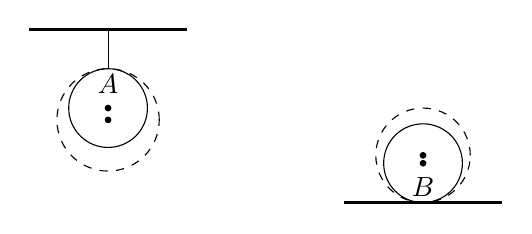
\begin{tikzpicture}
		\draw[very thick] (-4,0) -- (-2,0);
		\draw (-3,0) -- (-3,-.5);
		\draw (-3,-1) circle (.5);
		\draw[dashed](-3,-1.15) circle (.65);
		\node at (-3,-.7)  {$A$};
		\filldraw[black] (-3,-1) circle (1pt);
		\filldraw[black] (-3,-1.15) circle (1pt);
		\draw[very thick] (0,-2.2) -- (2,-2.2);
		\draw (1,-1.7) circle (.5);
		\draw[dashed] (1,-1.6) circle (.6);
		\filldraw[black] (1,-1.7) circle (1pt);
		\filldraw[black] (1,-1.6) circle (1pt);
		\node at (1,-2) {$B$}; 
	\end{tikzpicture}
\end{figure}\\
Durch die Wärmezufuhr dehnen sich die Kugeln aus. Gehen wir davon aus, dass die Kugel die Wärme langsam und aus allen Richtungen gleichmäßig verteilt zugeführt bekommt, können wir davon ausgehen, dass sich die Kugel auch gleichmäßig ausdehnt. Das bedeutet aber, dass sie ihre Form weiterhin beibehält.\footnote[2]{Vermutlich ist dies eine Folge der Rotationssymetrie der Anordnung und der gleichmäßigen Wärmezufuhr.}
Dadurch verschiebt sich nun aber der Kugelschwerpunkt. Es kann sich jedoch der Schwerpunkt der Kugel $A$ nur nach unten verschieben, und der Schwerpunkt der Kugel $B$ nur nach oben. \\
Verschiebt sich der Kugelschwerpunkt ändert sich auch die potentielle Energie im Gravitationsfeld der Erde. \\
Im Fall der Kugel $A$ verschiebt sich der Schwerpunkt nach unten. Das bedeutet aber, dass die potentielle Energie der Kugel geringer wird. \\
Gleichzeitig verschiebt sich der Schwerpunkt der Kugel $B$ weiter nach oben. Dadurch erhöht sich aber die potentielle Energie der Kugel. \\
Bei der Bewegung von Kugel $A$ kann diese \glqq verlorene\grqq{} potentielle Energie aber nicht einfach verschwinden, und bei der Kugel $B$ muss die \glqq gewonnen\grqq{} potentielle Energie irgendwo herkommen. \\
An dieser Stelle kann man ein Energieerhaltungsargument bringen, oder, wenn man genauer seien möchte, den \textit{1. Hauptsatz der Thermodynamik} verwenden. Dieser besagt
\end{Answer}
